% =====================================================================
% Scenario 4: Kubernetes Fault Tolerance & Rerouting
%
% Paste this block into your main document where the other scenarios sit.
% LaTeX will number the section and subsections automatically, so it will
% pick up whatever number follows Scenario 3.
%
% Required in your preamble:
%   \usepackage{graphicx}
%
% Required image (already generated in this folder):
%   docs/sequence-diagram-scenario4.png
% =====================================================================

\section{Scenario 4: Kubernetes Fault Tolerance \& Rerouting}

\subsection{Introduction}
This scenario simulates the sudden death of an entire machine inside a container
orchestrator cluster while that machine is actively serving live user traffic.
Three identical copies of an order backend run on three separate machines behind
a load balancer, so that no single machine is a point of failure. One of those
machines is then destroyed instantly, without warning, in the middle of
operation.

\textbf{The Goal:} The objective is to measure how a self-healing orchestrator
reroutes traffic and repairs itself, and then to train a predictive
(\textit{regression}) AI model that estimates the remaining time to full system
restabilization using only the first few seconds of the disturbance.

\textbf{Main Idea:} When a machine dies, the system does not fail all at once,
and it does not recover all at once. The damage arrives in two separate waves.
First comes a wave of \textit{failed} requests, because the load balancer does
not yet know the machine is gone and keeps confidently routing traffic to a
computer that no longer exists. Only after the orchestrator detects the loss and
removes that machine does the second wave arrive: a wave of extreme
\textit{slowness}, because the two surviving copies must now absorb all of the
traffic with only two thirds of the original capacity. The AI must learn the
shape of this two-wave recovery curve well enough to predict when the system
will be fully healthy again.

\subsection{System Model}
The model is a five-machine Kubernetes cluster. One machine runs the
orchestrator itself, one machine runs the observability tools and the entry
point, and three machines each run one copy of the order backend. The
observability machine is deliberately kept separate from the machines under
attack, so that the instrument measuring the failure can never be destroyed by
it.

The model rests on a strict capacity rule. Each copy of the backend can process
only two requests at the same time, and each request takes $0.1$ seconds, so a
single copy can serve $20$ requests per second. Three copies therefore serve
$60$ requests per second, and two copies serve only $40$ requests per second.
Traffic is offered at a constant $42$ requests per second. While all three
copies are alive the cluster runs at $70\%$ of capacity and is comfortable. The
moment one copy is lost the same traffic represents $105\%$ of the remaining
capacity, so a queue forms and waiting time grows for as long as the missing
copy is absent.

Three timing rules complete the model. The entry point abandons any request that
takes longer than $5.0$ seconds, which is what turns requests aimed at the dead
machine into recorded failures. The orchestrator waits roughly $40$ seconds of
missed heartbeats before it declares a machine dead, which is the length of the
first wave. Finally, a newly started copy refuses traffic for its first $15$
seconds while it warms up, which means a replacement is scheduled long before it
is actually useful.

Restabilization is defined precisely rather than by eye. The system counts as
fully recovered at the first second from which, for at least $8$ of the
following $10$ seconds, response time has returned to within $25\%$ of the
pre-failure baseline, the failure rate has returned to its normal level, and all
three copies are once again serving traffic.

\subsection{Sequence Diagram Description (Workflow):}
A steady stream of end users sends order requests to our Level 1 API Gateway,
which forwards each one through a load balancer that spreads the work evenly
across three copies of the Level 2 order backend. While this traffic is still
flowing, we inject the fault by instantly destroying the machine hosting the
third copy. For roughly the next $40$ seconds the orchestrator has not yet
noticed, so the load balancer keeps sending one third of all traffic to the dead
machine; those requests hang and are abandoned after $5$ seconds, and the user
receives a failure. Curiously, the requests that reach a living copy during this
same period are still perfectly fast, which makes the failure look confusing on
a dashboard. The orchestrator then detects the missed heartbeats, removes the
dead copy from the load balancer, and the failures stop immediately. However,
all of the traffic is now squeezed into two copies instead of three, so a queue
builds and the typical response time climbs from about $110$ milliseconds to
roughly $1{,}900$ milliseconds; nothing is broken, but everything is slow. In
parallel the orchestrator schedules a replacement copy on a surviving machine,
which needs a further $15$ seconds to warm up before it accepts any work. Once
it becomes ready the load balancer restores traffic across three copies, the
backlog drains, and response time returns to the original baseline. Throughout
this entire process OpenTelemetry silently records every single request as a
trace, including which copy and which machine served it, and ships those traces
to our Jaeger database. Our data pipeline then extracts these traces and
flattens them into a time series with one row per second of the incident.
Finally, our AI forecaster learns the shape of this recovery curve and reports
how much longer the healing will take.

\vspace{0.5em}
\noindent\textbf{SUMMARY OF WORKFLOW}
\begin{enumerate}
    \item \textbf{Steady User Traffic} $\rightarrow$ $42$ requests per second
          arrive at the Level 1 API Gateway.
    \item \textbf{Load Balancer} $\rightarrow$ spreads the work evenly across
          three copies of the Level 2 order backend.
    \item \textbf{Fault Injected} $\rightarrow$ the machine hosting the third
          copy is destroyed instantly, mid-operation.
    \item \textbf{Black Hole Phase (about 40 s)} $\rightarrow$ the load balancer
          still sends one third of traffic to the dead machine. Those requests
          are abandoned after $5$ seconds and marked as errors, while the
          surviving path stays fast.
    \item \textbf{Orchestrator Detects the Loss} $\rightarrow$ heartbeats are
          missed, the machine is declared dead, and its copy is removed from the
          load balancer. Failures stop.
    \item \textbf{Brownout Phase} $\rightarrow$ two copies now carry all of the
          traffic at $105\%$ of their capacity. A queue builds and response time
          climbs from about $110$ ms to about $1{,}900$ ms, with no errors at
          all.
    \item \textbf{Self-Healing} $\rightarrow$ the orchestrator schedules a
          replacement copy, which warms up for $15$ seconds before accepting
          traffic.
    \item \textbf{Restabilization} $\rightarrow$ traffic resumes across three
          copies, the backlog drains, and response time returns to baseline.
    \item \textbf{OpenTelemetry} $\rightarrow$ ships every request as a trace to
          Jaeger, recording the serving copy and machine for each one.
    \item \textbf{AI Forecaster} $\rightarrow$ analyses the recovery curve and
          predicts the remaining seconds until the system is fully stable.
\end{enumerate}

\begin{figure}[h]
    \centering
    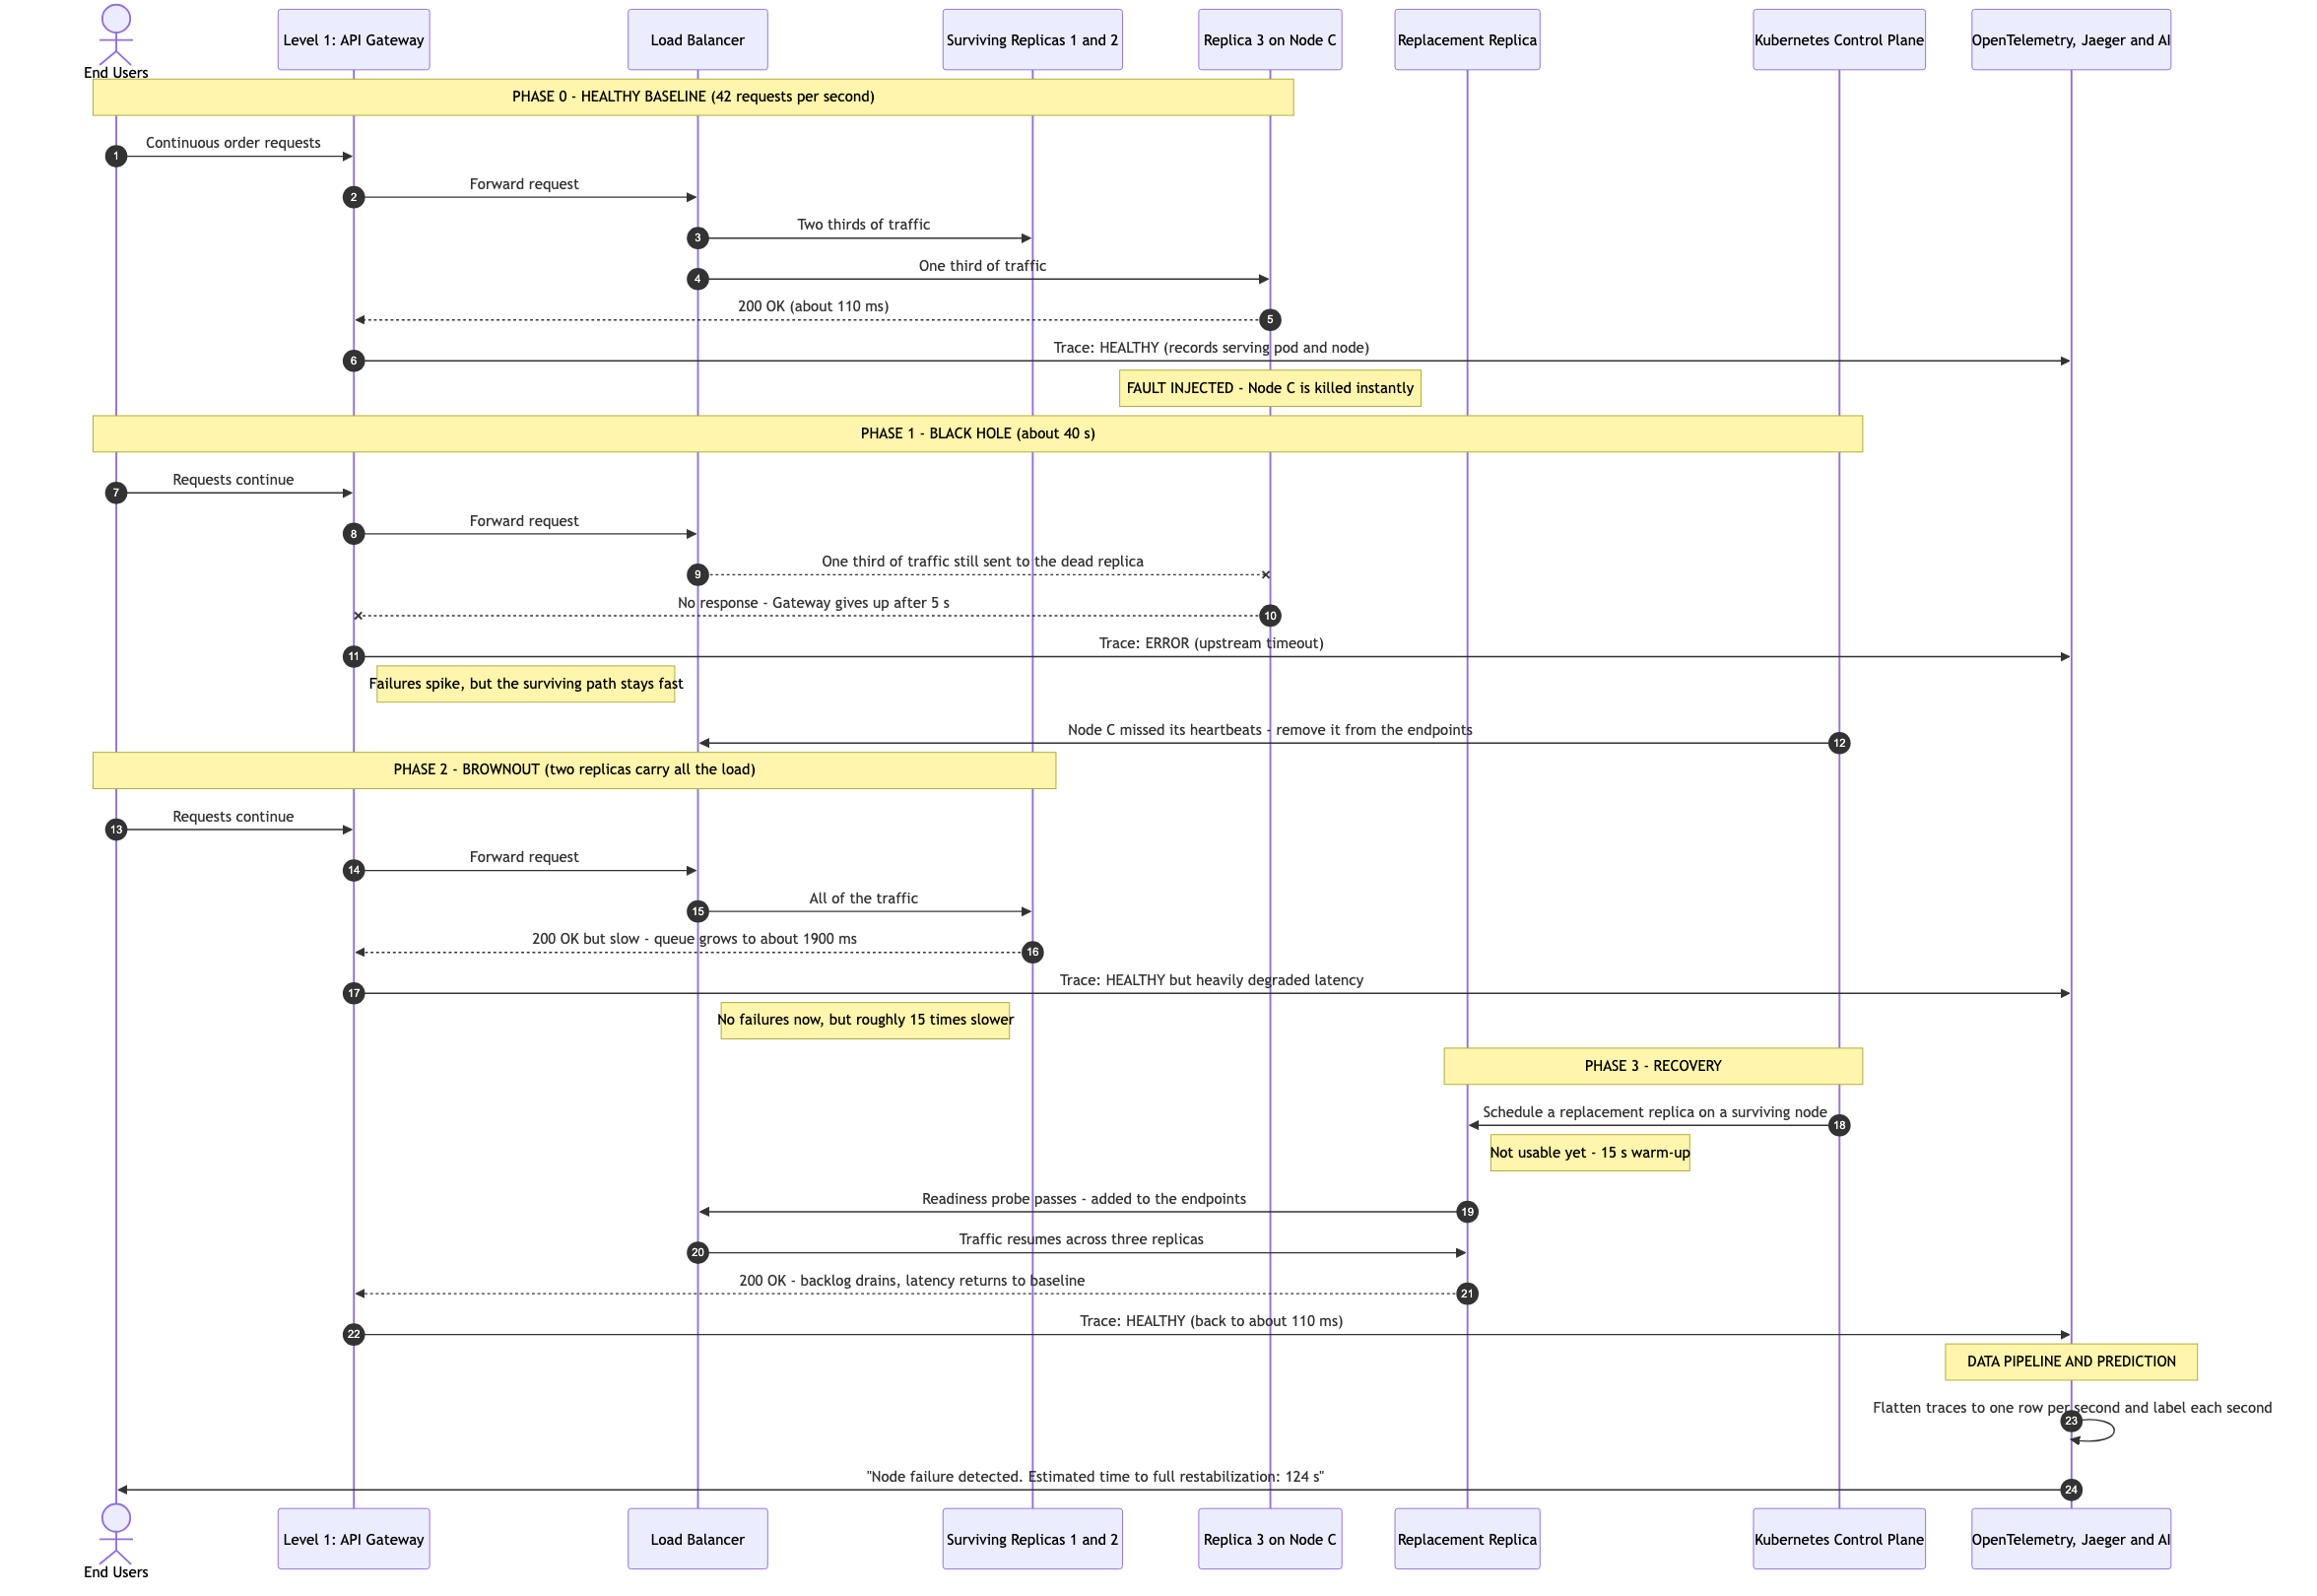
\includegraphics[width=\textwidth]{docs/sequence-diagram-scenario4.png}
    \caption{Sequence diagram for the Kubernetes node failure, traffic
    rerouting and restabilization scenario.}
    \label{fig:scenario4-sequence}
\end{figure}

\subsection{Scenario Implementation}
The cluster was implemented with \texttt{kind}, which runs a genuine
five-machine Kubernetes cluster locally. The order backend and the API Gateway
were written in Python and instrumented with the \texttt{opentelemetry-sdk},
exporting traces over OTLP to a Jaeger instance deployed inside the cluster. The
backend enforces its capacity limit with a counter that allows only
\texttt{WORKER\_SLOTS}$=2$ requests to be processed at once, each taking
\texttt{SERVICE\_TIME\_MS}$=100$; the time a request spends waiting for a free
slot is recorded on its trace and is the direct measurement of the queue.

Traffic was produced by an \textit{open-loop} load generator, which sends a
fixed $42$ requests per second regardless of how slow the system becomes. This
choice is essential: a closed-loop generator would automatically slow down as
the system slowed down, which would hide the brownout entirely. The fault was
injected at $60$ seconds into a $300$ second run by forcefully killing the
container that hosts one of the machines, so that the machine disappears without
any graceful shutdown, exactly like a pulled power cable.

Two orchestrator settings were tuned to keep the recovery inside a short
experiment. The tolerance for an unreachable machine was reduced from the
Kubernetes default of $300$ seconds to $10$ seconds, so that replacement copies
are created promptly. The anti-affinity rule that spreads the copies across
machines was made a preference rather than a requirement, so that the
replacement copy is always able to find somewhere to run instead of waiting
forever for the dead machine to return.

The data pipeline then extracted approximately $12{,}000$ traces per run from
Jaeger and flattened them into one row per second. Each row holds the
measurements an engineer would see on a dashboard, including the request rate,
the failure rate, the median and $95$th percentile response times, the mean
queue waiting time, and the number of distinct copies that actually served
traffic in that second. Each row was then labelled with the number of seconds
remaining until full restabilization, which converts the problem from
classification into regression. Across two recorded runs, full restabilization
took $88$ seconds and $134$ seconds respectively, and the $95$th percentile
response time peaked at between $24$ and $27$ times the healthy baseline.

\subsection{Evaluation}
A Random Forest Regressor, a Gradient Boosting Regressor and a Linear Regression
model were evaluated. Because a single incident produces only a single recovery
curve, the models were validated using \textit{leave-one-run-out} testing: the
model is trained on one complete outage and then asked to predict a different
outage it has never seen. On that basis the Random Forest predicted the remaining
time to restabilization with a mean absolute error of approximately $21$ seconds.

The evaluation was deliberately run twice, on two different sets of inputs, to
guard against a subtle form of cheating. Given the elapsed time since the
failure, a model can appear almost perfect simply by subtracting that number from
a memorised total, without understanding the system at all. The second
evaluation therefore removed the elapsed-time input and forced the model to rely
only on the shape of the response-time and copy-count curves; accuracy under
this stricter test was approximately $24$ seconds. The small gap between the two
figures confirms that the model is genuinely reading the recovery dynamics rather
than merely reading a clock. Inspection of the feature importances supports this,
showing that after elapsed time the model relies most heavily on the ratio of
current response time to the healthy baseline and on the mean queue waiting time.
